\documentclass[10pt]{exam}
\usepackage[phy]{template-for-exam}
\usepackage{hyperref,graphicx,enumitem}
\setlist[itemize]{topsep=0pt,itemsep=-1ex,partopsep=1ex,parsep=1ex}


\title{Air Rocket Lab - \\ \sc Launch Day Makeup Assignment}
\author{Rohrbach}
\date{\today}

\begin{document}
\maketitle


\noindent
Go to 

{\small \url{https://phet.colorado.edu/sims/html/projectile-motion/latest/projectile-motion_all.html}}

\noindent
Or go to Google and type in ``\texttt{projectile motion PhET}''

\begin{itemize}
  \item Go to the ``Intro'' tab.
  \item Drag the cannon to the ground (altitude of 0 m)	and drag the target to 11.0 meters
  
  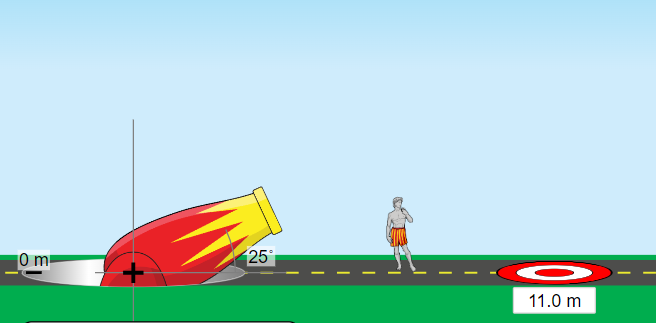
\includegraphics[width=7cm]{cannon.png} 
\end{itemize}


\section*{Purpose}
 Your goal is to hit the target at 11 meters in three shots of the cannon.  You can only change the angle of each shot, you cannot change the initial speed (it should remain at 15 m/s).

\section*{Pre-Lab}

\begin{questions}


  \question
    Think, if your first launch goes too far, what do you think you should do to the angle of your second shot?  What about if your launch goes too short?
    \vspace{5em}

  
\end{questions}

\section*{Launches}

\subsection*{Trial 1 - the test shot:}

\noindent
What angle did you use?
\vspace{5em}

\noindent
Describe what happened. (Did it go too far, too short)
\vspace{5em}

\noindent
What angle will you use for your second shot?  Why?  (Make sure to think about what we've talked about in class in terms of how angles affect the range of a projectile.)
\vspace{5em}


\subsection*{Trial 2 - adjustments:}
\noindent
What angle did you use?
\vspace{5em}

\noindent
Describe what happened. (Did it go too far, too short)
\vspace{5em}

\noindent
What angle will you use for your third shot?  Why?  (Make sure to think about what we've talked about in class in terms of how angles affect the range of a projectile.)
\vspace{5em}




\subsection*{Trial 3 - make it happen:}

\noindent
What angle did you use?
\vspace{5em}

\noindent
Describe what happened. (Did it go too far, too short)
\vspace{5em}


			
\section*{Conclusions}
Write a few sentences to answer the following questions:

a.	What was the purpose of this lab? 

b.	Were you successful?  Why or why not? 



\end{document}